\documentclass[../TST.tex]{subfiles}
\begin{document}
\begin{large}
	\textbf{Short Exam 2}
\end{large}

\begin{sproblem}[Efficiency of a circuit]
Consider the circuit on Figure \ref{fig1}. The voltage source, the ammeters, and the voltmeter are ideal. The resistances $R_1$ and $R_2$ are constant, while the resistance $R_x$ may vary between zero and infinity. The efficiency of the circuit $\eta$ is defined as the ratio of the power dissipated at $R_x$ to the total power dissipated in the circuit.
\begin{subpart}
	\item Find an expression for $\eta$ in terms of $R_1$, $R_2$, and $R_x$. \score{2.5}
	\item Find the value of $R_x$ which maximizes $\eta$, in terms of $R_1$ and $R_2$. \score{1.5}
	\item Find an expression for the maximum $\eta$ in terms of the ratio $k=R_2/R_1$. \score{0.5}
	\item Find the value of $\eta$ (in percent) for $k=1$.\score{0.5} \\
\end{subpart}

\begin{figure}[h]
\centering
% \hspace*{0.6cm}
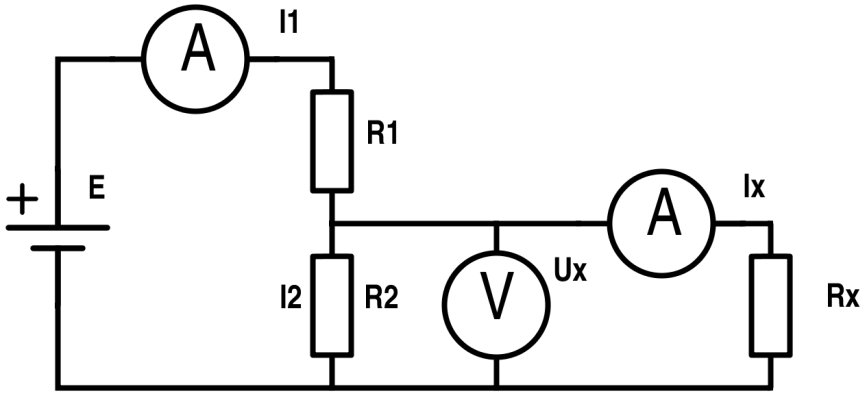
\includegraphics[width=0.6\textwidth]{fig/2015_l2.png}
\caption{}
\label{fig1}
\end{figure}
\end{sproblem}

\ifprob \else
	\begin{solution} (a) Firstly, let's note that there will be no power dissipation at the ammeters and voltmeters because their resistances are zero and infinity, respectively. Now, using the notation on the diagram, the power at $R_x$ is $U_xI_x$, while the power for the whole circuit equals the power supplied by the battery, which is $EI_1$. Then we have $\eta=\frac{U_xI_x}{EI_1}$, and all that is left is to find how the currents and voltages are related.  The current $I_1$ will split into $I_x$ and $I_2=I_1-I_x$, such that $I_xR_x=I_2R_2$. It follows that $I_x=\frac{I_1R_2}{R_x+R_2}$, which brings us to $\eta = \frac{R_2}{R_x+R_2}\frac{U_x}{E}$. The equivalent resistance of $R_2$ and $R_x$ is $R_\mathrm{eq}=\frac{R_2R_x}{R_2+R_x}$. The voltage drop at $R_\mathrm{eq}$ is $U_x=\frac{ER_\mathrm{eq}}{R_1+R_\mathrm{eq}}$, and thus
		\begin{equation*}
			\eta = \frac{R_2}{R_x+R_2}\cdot \frac{R_\mathrm{eq}}{R_1+R_\mathrm{eq}}= \boxed{\frac{R_2^2R_x}{(R_2+R_x)(R_1R_2+R_1R_x+ R_2R_x)}.}
		\end{equation*}
		(b) The efficiency $\eta$ is maximised when its inverse $1/\eta$ is minimised. Equivalently, we want to maximise
		\begin{equation*}
		\left(\frac{R_2}{R_x}+1\right) \left(R_x(R_1+R_2)+R_1R_2\right) 
		.
		\end{equation*}
The part of this expression that depends on $R_x$ is 
\begin{equation*}
\left(\frac{R_2}{R_x}\right) R_1R_2+R_x(R_1+R_2)
.
\end{equation*}
Now we can either take the derivative or use the AM-GM inequality to find that the expression is minimised when the two terms are equal, which happens at
\begin{equation*}
	\boxed{R_x=\sqrt{\frac{R_1}{R_1+R_2}}R_2.}
\end{equation*}
(c) We substitute $R_1=\frac{R_2}{k}$ and $R_x=\frac{R_2}{\sqrt{1+k}}$ into the expression for $\eta$. After some tedious manipulations, we get
\begin{equation*}
	\boxed{\eta = \frac{k}{2\sqrt{1+k}+(2+k)}.}
\end{equation*}
(d) The answer is 
\begin{equation*}
	\eta = \frac{1}{3+2\sqrt{2}} = \boxed{\qty{17.2}{\percent}.}
\end{equation*}
If you have time, it's a good idea to solve the special case $k=1$ separately and confirm that the numerical answer is in agreement with the general formula.

\end{solution}
\fi
\ifprob 
	\clearpage
\else 
	\vspace*{10mm}
	% \clearpage
\fi
\end{document}

